% !Tex program = pdflatex
% 第 0 章: 代数学基础
\ifx\allfiles\undefined
\documentclass{note}
\begin{document}
\setcounter{chapter}{-1}
\fi
\chapter{代数学基础}
\section{常用符号}
\begin{itemize}
    \item $\forall$: 对所有 (for all).
    \item $\exists$: 存在 (there exists).
    \item $\exists!$: 存在且唯一 (there exists exactly one).
    \item s.t.: 使得 (such that).
    \item $\mathbb{N}$: 自然数.
    \item $\mathbb{Z}$: 整数.
    \item $\mathbb{Q}$: 有理数.
    \item $\mathbb{R}$: 实数.
    \item $\mathbb{C}$: 复数.
\end{itemize}

\section{集合}
\begin{df}[集合 (Set)]
\end{df}

\textbf{元素与集合之间的关系}: 对元素 $a$ 和集合 $S$,
\begin{itemize}
    \item $a\in S$ 或
    \item $a\notin S$.
\end{itemize}

\textbf{集合中元素之间的关系}: $\forall a,b\in S$,
\begin{itemize}
    \item $a=b$ 或
    \item $a\neq b$.
\end{itemize}

\textbf{集合与集合之间的关系}: 对集合 $A,B$ 和全集 $I$,
\begin{itemize}
    \item[(1)] \textbf{交集}: $A\cap B=\{a\mid a\in A\text{ 且 }a\in B\}$.
    \item[(2)] \textbf{并集}: $A\cup B=\{a\mid a\in A\text{ 或 }a\in B\}$.
    \item[(3)] \textbf{差}: $B-A=\{a\mid a\in B\text{ 且 }a\notin A\}$.
    \item[(4)] \textbf{补集}: $A'=I-A=\{a\mid a\in I\text{ 且 }a\notin A\}$.
    \item[(5)] \textbf{包含}: $A\subseteq B$, 称 $A$ 包含于 $B$, 或称 $B$ 包含 $A$, 或称 $B$ 是 $A$ 的子集\\
    $\Longleftrightarrow A\cup B=A\Longleftrightarrow A\cup B=B$.
    \begin{pf}
        \uline{$A\subseteq B\Longrightarrow A\cap B=A$}: $\because A\subseteq B$, $\therefore\forall a\in A$, $a\in B\Longrightarrow A\subseteq A\cap B$.\\
        $\forall a\in A\cup B$, 由交集定义, $a\in A\Longrightarrow A\cap B\subseteq A$.\\
        故 $A\cap B=A$.

        \uline{$A\subseteq B\Longleftarrow A\cap B=A$}: $\because A\cap B=A$, $\therefore\forall a\in A$, $a\in B\Longrightarrow A\subseteq B$.

        \uline{$A\subseteq B\Longrightarrow A\cup B=B$}: $\because A\subseteq B$, $\forall a\in A$, $a\in B$, $\therefore\forall a\in A\cup B$, $a\in B\Longrightarrow A\cup B\subseteq B$.\\
        $\because A\subseteq B$, $\forall a\in A$, 由并集定义, $a\in A\cup B\Longrightarrow B\subseteq A\cup B$.\\
        故 $A\cup B=B$.

        \uline{$A\subseteq B\Longleftarrow A\cup B=B$}: $\forall a\in A$, 由并集定义, $a\in A\cup B$, 又 $\because A\cup B=B$, $\therefore a\in B\Longrightarrow A\subseteq B$.

        综上, 得证.
    \end{pf}
\end{itemize}

\textbf{常用公式}:
\begin{itemize}
    \item[(1)] $A\cap(\cup_i B_i)=\cup_i(A\cap B_i)$.
    \begin{pf}
        $\forall a\in A(\cup_i B_i)\Longleftrightarrow a\in A$ 且 $a\in \cup_iB_i$\\
        $\Longleftrightarrow a\in A$ 且 $\exists k$, s.t. $a\in B_k$\\
        $\Longleftrightarrow\exists k$, s.t. $a\in A\cap B_k\subseteq\cup_i(A\cap B_i)$\\
        $\Longleftrightarrow a\in\cup_i(A\cap B_i)$, 故 $A\cap(\cup_iB_i)\subseteq\cup_i(A\cap B_i)$.

        $\forall a\in\cup_i(A\cap B_i)\Longleftrightarrow\exists k$, s.t. $a\in A\cap B_k$\\
        $\Longleftrightarrow\exists k$, s.t. $a\in A$ 且 $a\in B_k$\\
        $\Longleftrightarrow a\in A$ 且 $\exists k$, s.t. $a\in B_k$\\
        $\Longleftrightarrow a\in A$ 且 $a\in\cup_iB_i$\\
        $\Longleftrightarrow a\in A\cap(\cup_iB_i)$, 故 $\cup_i(A\cap B_i)\subseteq A\cap(\cup_iB_i)$.

        综上, 得证.
    \end{pf}
    \item[(2)] $A\cup(\cap_iB_i)=\cap_i(A\cup B_i)$.
    \begin{pf}
        $\forall a\in A\cup(\cap_iB_i)\Longleftrightarrow a\in A$ 或 $a\in\cap_iB_i$\\
        $\Longleftrightarrow a\in A$ 或 $\forall i$, s.t. $a\in B_i$\\
        $\Longleftrightarrow\forall i$, $a\in A$ 或 $a\in B_k$\\
        $\Longleftrightarrow\forall i$, $a\in A\cup B_k$\\
        $\Longleftrightarrow\cap_i(A\cup B_i)$, 故 $A\cup(\cap_iB_i)\subseteq\cap_i(A\cup B_i)$.

        $\forall a\in\cap_i(A\cup B_i)\Longleftrightarrow\forall i$, $a\in A\cup B_i$\\
        $\Longleftrightarrow\forall i$, $a\in A$ 或 $a\in B_i$\\
        $\Longleftrightarrow a\in A$ 或 $\forall i$, $a\in B_i$\\
        $\Longleftrightarrow a\in A$ 或 $a\in\cup_iB_i$\\
        $\Longleftrightarrow a\in A\cap(\cup_iB_i)$, 故 $\cap_i(A\cup B_i)\subseteq A\cap(\cup_iB_i)$.

        综上, 得证.
    \end{pf}
    \item[(3)] $(\cup_iA_i)'=\cap_iA_i'$.
    \begin{pf}
        $\forall a\in(\cup_iA_i)'\Longleftrightarrow a\in I$ 且 $a\notin\cup_iA_i$\\
        $\Longleftrightarrow a\in I$ 且 $\forall i$, $a\notin A_i$\\
        $\Longleftrightarrow\forall i$, $a\in I$ 且 $a\notin A_i$\\
        $\Longleftrightarrow\forall i$, $a\in A_i'$\\
        $\Longleftrightarrow a\in\cap_iA_i'$, 故 $(\cup_iA_i)'\subseteq\cap_iA_i'$.

        $\forall a\in\cap_iA_i'\Longleftrightarrow\forall i$, $a\in I$ 且 $a\notin A_i$\\
        $\Longleftrightarrow a\in I$ 且 $\forall i$, $a\notin A_i$\\
        $\Longleftrightarrow a\in I$ 且 $a\notin\cup_iA_i'$\\
        $\Longleftrightarrow a\in(\cup_iA_i)'$, 故 $\cap_iA_i'\in(\cup_iA_i)'$.

        综上, 得证.
    \end{pf}
    \item[(4)] $(\cap_iA_i)'=\cup_iA_i'$.
    \begin{pf}
        $\forall a\in(\cap_iA_i)'\Longleftrightarrow a\in I$ 且 $a\notin\cap_iA_i$\\
        $\Longleftrightarrow a\in I$ 且 $\exists k$, s.t. $a\notin A_k$\\
        $\Longleftrightarrow\exists k$, s.t. $a\in I$ 且 $a\notin A_k$\\
        $\Longleftrightarrow\exists k$, s.t. $a\in A_k'$\\
        $\Longleftrightarrow a\in\cup_iA_i'$, 故 $(\cap_iA_i)'\subseteq\cup_iA_i'$.

        $\forall a\in\cup_iA_i'\Longleftrightarrow\exists k$, s.t. $a\in A_k'$\\
        $\Longleftrightarrow\exists k$, s.t. $a\in I$ 且 $a\notin A_k$\\
        $\Longleftrightarrow a\in I$ 且 $\exists k$, s.t. $a\notin A_k$\\
        $\Longleftrightarrow a\in I$ 且 $a\notin\cap_iA_i$\\
        $\Longleftrightarrow a\in(\cap_iA_i)'$, 故 $\cup_iA_i'\subseteq(\cap_iA_i)'$.

        综上, 得证.
    \end{pf}
\end{itemize}

\section{映射}
\begin{df}[映射]
    $\forall a\in S_1$, $\exists!b\in S_2$, s.t. $b=f(a)$, 记作 $f:S_1\rightarrow S_2$, $a\mapsto b$, 其中称 $S_1$ 为定义域, $S_2$ 为值域, $b$ 为 $a$ 的像, $a$ 为 $b$ 的原像.
\end{df}

\begin{eg}[恒等映射]
    $1_S:S\rightarrow S$, $a\mapsto 1_S(a)=a$.
\end{eg}

\begin{df}[映射相等]
    映射 $f:S_1\rightarrow S_2$, $g:S_1\rightarrow S_3$, $\forall a\in S_1$, $f(a)=g(a)$, 则称 $f$ 与 $g$ 相等, 记作 $f=g$.
\end{df}

$\forall a\in S_1$, $\{f(a)\}\subseteq S_2$ 且 $\abs{\{f(a)\}}=1$.

\begin{df}[原像集]
    $f^{-1}(b)\equiv\{a\in S_1\mid f(a)=b\}$.
\end{df}

$f^{-1}(b)\subseteq S_1$, $f^{-1}(b)$ 可能 $=\emptyset$.

\begin{df}[像集]
    $\im f=f(S_1)\equiv\{b\in S_2\mid b=f(a)\forall a\in S_1\}$.
\end{df}

$\im f\subseteq S_2$.

\textbf{基本性质}:
\begin{itemize}
    \item[(1)] $A\subseteq S_1\Longrightarrow A\subseteq f^{-1}(f(A))$.
    \begin{pf}
        $\forall a\in A$, $\because A\subseteq S_1$, $\therefore a\in S_1$.\\
        又 $\because f(a)\in f(A)$, $\therefore a\in f^{-1}(f(A))$, 故 $A\subseteq f^{-1}(f(A))$.
    \end{pf}

    若 $\exists a\in S_1-A$, s.t. $f(a)\in f(A)$, 则 $A\subsetneq f^{-1}(f(A))$.
    \item[(2)] $B\subseteq S_2\Longrightarrow B\supseteq f(f^{-1}(B))$.
    \begin{pf}
        $\because f^{-1}(B)=\{a\in S_1\mid f(a)\in B\}$, $\therefore\forall a\in f^{-1}(B)$, $f(a)\in B\Longrightarrow f(f^{-1}(B))\subseteq B$.
    \end{pf}

    若 $\exists b\in B$, s.t. $\forall a\in S_1$, $f(a)\neq b$ (即 $B$ 中有元素在 $S_1$ 中无原像), 则 $B\supsetneq f(f^{-1}(B))$.

    若 $\forall b\in B$, $\exists a\in A$, s.t. $f(a)=b$, 则 $B=f(f^{-1}(B))$.
    \item[(3)] $f^{-1}(\cup_iB_i)=\cup_if^{-1}(B_i)$.
    \begin{pf}
        $\forall a\in f^{-1}(\cup_iB_i)$, $\exists k$, s.t. $f(a)\in B_k$\\
        $\Longleftrightarrow\exists k$, s.t. $a\in f^{-1}(B_k)$\\
        $\Longleftrightarrow a\in\cup_if^{-1}(B_i)$, 故 $f^{-1}(\cup_iB_i)\subseteq\cup_if^{-1}(B_i)$.

        $\forall a\in\cup_if^{-1}(B_i)$, $\exists k$, s.t. $a\in f^{-1}(B_k)$\\
        $\Longleftrightarrow\exists k$, s.t. $f(a)\in B_k$\\
        $\Longleftrightarrow f(a)\in\cup_iB_i$\\
        $\Longleftrightarrow a\in f^{-1}(\cup_iB_i)$, 故 $\cup_if^{-1}(B_i)\subseteq f^{-1}(\cup_iB_i)$.

        综上, 得证.
    \end{pf}
    \item[(4)] $f^{-1}(\cap_iB_i)=\cap_if^{-1}(B_i)$.
    \begin{pf}
        $\forall a\in f^{-1}(\cap_iB_i)$, $\exists k$, s.t. $f(a)\in B_k$\\
        $\Longleftrightarrow\exists k$, s.t. $a\in f^{-1}(B_k)$\\
        $\Longleftrightarrow a\in\cup_if^{-1}(B_k)$, 故 $f^{-1}(\cap_iB_i)\subseteq\cap_if^{-1}(B_i)$.

        $\forall a\in\cap_if^{-1}(B_i)$, $\forall i$, s.t. $a\in f^{-1}(B_i)$\\
        $\Longleftrightarrow\forall i$, s.t. $f(a)\in B_i$\\
        $\Longleftrightarrow f(a)\in\cap_iB_i$\\
        $\Longleftrightarrow a\in f^{-1}(\cap_iB_i)$, 故 $\cap_if^{-1}(B_i)\subseteq f^{-1}(\cap_iB_i)$.

        综上, 得证.
    \end{pf}
\end{itemize}

\begin{df}[映射的复合]
    映射 $f:S_1\rightarrow S_2$, $g:S_2\rightarrow S_3$, 则称映射 $g\circ f:S_1\rightarrow S_2$, $a\mapsto g\circ f(a)\equiv g(f(a))$ 为 $f$ 和 $g$ 的复合.
\end{df}

\begin{thm}[映射复合的结合律]
    $h\circ(g\circ f)=(h\circ g)\circ f$.
\end{thm}

故连续复合 $f_1\circ f_2\circ\cdots\circ f_n$ 无需括号.

\begin{df}[交换图]
    $f: S_1\rightarrow S_1$, $h:S_2\rightarrow S_3$, $g:S_1\rightarrow S_3$, 若 $g=f\circ h$, 则称该图交换.
    \begin{center}
        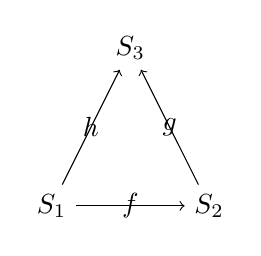
\begin{tikzpicture}
            \node(1)at(0,0){$S_1$};
            \node(2)at(2,0){$S_2$};
            \node(3)at(1,2){$S_3$};
            \draw[->](1)--(2)node[midway]{$f$};
            \draw[->](2)--(3)node[midway]{$g$};
            \draw[->](1)--(3)node[midway]{$h$};
        \end{tikzpicture}
    \end{center}

    $f:S_1\rightarrow S_2$, $g:S_2\rightarrow S_4$, $h:S_1\rightarrow S_3$, $l:S_3\rightarrow S_4$, 若 $g\circ f=l\circ h$, 则称该图交换.
    \begin{center}
        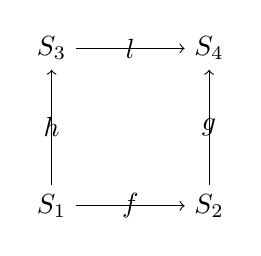
\begin{tikzpicture}
            \node(1)at(0,0){$S_1$};
            \node(2)at(2,0){$S_2$};
            \node(3)at(0,2){$S_3$};
            \node(4)at(2,2){$S_4$};
            \draw[->](1)--(2)node[midway]{$f$};
            \draw[->](2)--(4)node[midway]{$g$};
            \draw[->](1)--(3)node[midway]{$h$};
            \draw[->](3)--(4)node[midway]{$l$};
        \end{tikzpicture}
    \end{center}
\end{df}

\begin{df}[单射 (Injective 或 One-to-one)]
    映射 $f:S_1\rightarrow S_2$, $\forall a,b\in S_1$, 若 $f(a)=f(b)\Longrightarrow a=b$, 则称 $f$ 单射.
\end{df}

\textbf{单射的性质}:
\begin{itemize}
    \item[(1)] $c\in S_2$, $f$ 单射, 若 $f^{-1}(c)\neq\emptyset$, 则 $\abs{f^{-1}(c)}=1$.
    \item[(2)] $f$ 单射 $\Longleftrightarrow A=f^{-1}(f(A))$.
\end{itemize}

\begin{df}[满射 (Surjective)]
    映射 $f:S_1\rightarrow S_2$, 若 $\forall b\in S_2$, $\exists a\in S_1$, s.t. $f(a)=b$ (即 $\im f=S_2$), 则称 $f$ 满射.
\end{df}

\textbf{满射的性质}:
\begin{itemize}
    \item[(1)] $f$ 满射 $\Longleftrightarrow\forall B\subseteq S_2$, $f^{-1}(B)\neq\emptyset$.
    \item[(2)] $f$ 满射 $\Longleftrightarrow\forall B\subseteq S_2$, $B=f(f^{-1}(B))$.
\end{itemize}

\begin{df}[双射]
    映射 $f$ 单射且满射 $\Longleftrightarrow f$ 双射.
\end{df}

\begin{eg}
    恒等映射是双射的.
\end{eg}

\textbf{常用结论}:
\begin{itemize}
    \item[(1)] $f,g$ 单射 $\Longrightarrow g\circ f$ 单射.
    \begin{pf}
        $\forall a,b\in S_1$, 若 $g\circ f(a)=g\circ f(b)$, $\because g$ 单射, $\therefore f(a)=f(b)$,\\
        又 $\because f$ 单射, $\therefore a=b$, 故 $g\circ f$ 单射.
    \end{pf}
    \item[(2)] $g\circ f$ 单射 $\Longrightarrow f$ 单射.
    \begin{pf}
        $\forall a,b\in S_1$, 若 $f(a)=f(b)$, 则 $g\circ f(a)=g\circ f(b)$,\\
        又 $\because g\circ f$ 单射, $\therefore a=b$, 故 $f$ 单射.
    \end{pf}

    \begin{eg}[$g\circ f$ 单射, 而 $g$ 非单射的例子]
        集合 $S_1=\{0\}$, $S_2=\{0,1\}$, $S_3=\{0\}$,\\
        映射 $f:S_1\rightarrow S_2$, $f(a)=0\forall a\in S_1$, 单射,\\
        $g:S_2\rightarrow S_3$, $g(b)=0\forall S_2$, 非单射,
        $g\circ f:S_1\rightarrow S_3$, $g(a)=0$, 单射.
    \end{eg}
    \item[(3)] $f,g$ 满射 $\Longrightarrow g\circ f$ 满射.
    \begin{pf}
        $\forall c\in S_3$, $\because g$ 满射, $\therefore\exists b\in S_2$, s.t. $g(b)=c$,\\
        又 $\because f$ 满射, $\therefore\exists a\in S_1$, s.t. $f(a)=b\Longrightarrow g\circ f(a)=c$, 故 $g\circ f$ 满射.
    \end{pf}
    \item[(4)] $g\circ f$ 满射 $\Longrightarrow g$ 满射.
    \begin{pf}
        $\because g\circ f$ 满射, $\therefore\forall c\in S_3$, $\exists a\in S_1$, s.t. $g\circ f(a)=c$\\
        $\Longrightarrow\exists b=f(a)\in S_2$, s.t. $g(b)=c$, 故 $g$ 满射.
    \end{pf}

    \begin{eg}[$g\circ f$ 满射, 而 $f$ 非满射的例子]
        集合 $S_1=\{0\}$, $S_2=\{0,1\}$, $S_3=\{0\}$,\\
        映射 $f:S_1\rightarrow S_2$, $f(a)=0\forall a\in S_1$, 非满射,\\
        $g:S_2\rightarrow S_3$, $g(b)=0\forall S_2$, 满射,
        $g\circ f:S_1\rightarrow S_3$, $g(a)=0$, 满射.
    \end{eg}
\end{itemize}

\begin{thm}\label{left inverse}
    映射 $f:S_1\rightarrow S_2$ 单射 $\Longleftrightarrow\exists$ 映射 $g:S_2\rightarrow S_1$, s.t. $g\circ f=1_{S_1}$, 这样的 $g$ 称为 $f$ 的左逆.
\end{thm}
\begin{pf}
    ``$\Longrightarrow$'': 构造 $g(b)=\left\{\begin{array}{ll}
        a,&a\in f^{-1}(b),\\
        \text{任意取一个 }a_0\in S_1,&f^{-1}(b)=\emptyset,
    \end{array}\right.$,\\
    $\forall a\in S_1$, 记 $b=f(a)$, $\because f$ 单射且 $a\in f^{-1}(b)\neq\emptyset$, $\therefore\abs{f^{-1}(b)}=1$,\\
    $\Longrightarrow g\circ f(a)=a\Longrightarrow g\circ f=1_{S_1}$.

    ``$\Longleftarrow$'': $\forall a,b\in S_1$, 若 $f(a)=f(b)$, 则 $a=1_{S_1}=g\circ f(a)=g\circ f(b)=1_{S_1}(b)=b$, 故 $f$ 单射.
\end{pf}

由于当 $f^{-1}(b)=\emptyset$ 时, $g(b)$ 的取值具有任意性, 故若左逆存在, 则不唯一.

\begin{thm}\label{right inverse}
    映射 $f:S_1\rightarrow S_2$ 满射 $\Longleftrightarrow\exists$ 映射 $h:S_2\rightarrow S_1$, s.t. $f\circ h=1_{S_2}$, 这样的 $h$ 称为 $f$ 的右逆.
\end{thm}
\begin{pf}
    ``$\Longrightarrow$'': $\because f$ 满射, $\therefore\forall b\in S_2$, $\exists a\in S_1$, s.t. $f(a)=b$, 故可构造 $h(b)=a\in f^{-1}(b)$,\\
    从而 $f\circ h(b)=b\Longrightarrow f\circ h=1_{S_2}$.

    ``$\Longleftarrow$'': $\forall b\in S_2$, $\exists a=h(b)\in S_1$, s.t. $f\circ h(b)=1_{S_2}(b)=b$, 故 $f$ 满射.
\end{pf}

由于 $\abs{f^{-1}(b)}\geq 1$, $h(b)$ 的取值可能具有任意性, 故若右逆存在, 则不唯一.

\begin{thm}
    若映射 $f$ 同时存在左逆和右逆, 则其左逆 $=$ 右逆, 此时称 $f$ 可逆, 且此时 $f$ 双射.
\end{thm}
\begin{pf}
    因为 $f$ 同时存在左逆和右逆, 由定理 \ref{left inverse} 和 \ref{right inverse} 得 $f$ 双射.\\
    设左逆 $g:S_2\rightarrow S_1$, s.t. $g\circ f=1_{S_1}$, 右逆 $h:S_2\rightarrow S_1$, s.t. $f\circ h=1_{S_2}$.\\
    假设 $g\neq h$, 则 $\exists b\in S_2$, s.t. $g(b)\neq h(b)$,\\
    又 $\because f$ 单射, $\therefore b=1_{S_2}(b)=f\circ g(b)\neq f\circ h(b)$.\\
    $\because f$ 满射, $\therefore\exists a\in S_1$, s.t. $b=f(a)\Longrightarrow f(a)=b\neq f\circ g\circ f(a)=1_{S_2}(f(a))=f(a)$, 这显然是荒谬的, 故假设错误, $g=h$.
\end{pf}

\section{等价关系和等价类}
\begin{df}[卡氏积]
    集合 $S_1$ 和 $S_2$ 的卡氏积 $S_1\times S_2\equiv\{(a,b)\mid a\in S_1,b\in S_2\}$.\\
    集合 $S$ 的卡氏积 $S\times S\equiv\{(a,b)\mid a,b\in S\}$.
\end{df}
注意, 一般 $(a,b)\neq (b,a)$.

\begin{df}[关系]
    卡氏积的子集. $\mathcal{R}\in S\times S$, 称为 $S$ 上的关系.
\end{df}

\begin{eg}
    自然数集 $\mathbb{N}$ 的卡氏积 $\mathbb{N}\times\mathbb{N}=\{(n,m)\mid n,m\in\mathbb{N}\}$.

    小于关系: $\mathcal{R}_1=\{(n,m)\mid n-m<0\}$. $(1,2)\in\mathcal{R}_1$, 记作 $1\mathcal{R}_12$.

    等于关系: $\mathcal{R}_2=\{(n,m)\mid n-m=0\}$. $(1,1)\in \mathcal{R}_2$, 记作 $1\mathcal{R}_21$.
\end{eg}

\begin{df}[图]
    对映射 $f:S_1\rightarrow S_2$, 有关系 $G_f=\{(a,f(a))\mid a\in S_1\}\subseteq S_1\times S_2$, 称 $G_f$ 为 $f$ 的图.
\end{df}
(第一个坐标在此关系中仅出现一次, 不会重复.)

映射与图一一对应.

\begin{df}[等价关系]
    关系 $\mathcal{R}\in S\times S$, 若满足
    \begin{itemize}
        \item[(1)] \textbf{反身性}: $\forall a\in S$, $(a,a)\in\mathcal{R}$ (即 $a\sim a\forall a\in S$)
        \item[(2)] \textbf{对称性}: 若 $(a,b)\in\mathcal{R}$, 则 $(b,a)\in\mathcal{R}$ (即$a\sim b\Longleftrightarrow b\sim a$)
        \item[(3)] \textbf{传递性}: 若 $(a,b)\in\mathcal{R}$, $(b,c)\in\mathcal{R}$, 则 $(a,c)\in\mathcal{R}$ (即$a\sim b,b\sim c\Longleftrightarrow a\sim c$)
    \end{itemize}
    则称 $\mathcal{R}$ 为 $S$ 上的等价关系. 若元素 $a,b$ 具有等价关系, 记为 $a\sim b$.
\end{df}

\begin{df}[等价类]
    由具有等价关系的元素组成的集合. $\forall a\in S$, $[a]\equiv\{b\in S\mid b\sim a\}\subseteq$ 称为 $a$ 的等价类, $a$ 称为该等价类的代表元.
\end{df}

$\because a\in[a]$, $\therefore[a]$ 非空.

$c\in S$, 则有且仅有以下两种情况:
\begin{itemize}
    \item[(1)] $c\in[a]\Longleftrightarrow c\sim a\Longleftrightarrow a\sim c\Longleftrightarrow a\in[c]\Longleftrightarrow[a]=[c]$.
    \item[(2)] $c\notin[a]\Longleftrightarrow[a]\cap[c]=\emptyset$.
\end{itemize}
\begin{pf}
    假设 $[a]\cap[b]\neq\emptyset$, 则 $\exists c\in[a]\cap[b]$\\
    $\Longleftrightarrow c\in[a]$ 且 $c\in[b]$, 即 $c\sim a$ 且 $c\sim b$\\
    $\Longrightarrow a\sim b\Longrightarrow[a]=[b]$, 得证.
\end{pf}

\textbf{等价类的性质}
\begin{itemize}
    \item[(1)] $a\in[b]\Longleftrightarrow b\in[a]\Longleftrightarrow[a]=[b]$.
    \item[(2)] $a\notin[b]\Longleftrightarrow[a]\cap[b]=\emptyset$.
    \item[(3)] $\forall a,b\in S$, 要么 $[a]=[b]$, 要么 $[a]\cap[b]=\emptyset$.\\
    (以上三条证明见前文.)
    \item[(4)] $S=\cup_{i\in K,a_i\in S}[a_i]$, 其中 $[a_i]\cap[a_j]=\emptyset\forall i\neq j$.
    \begin{pf}
        $S=\cup_a\{a\}$, 合并各等价类, 即得证.
    \end{pf}
\end{itemize}

等价类这一概念可用于将大问题分解为小问题加以解决.

\begin{df}[剖分]
    集合 $S\neq\emptyset$, 若 $S=\cup_{i\in K,S_i\subseteq S}S_i$ 且 $S_i\cap S_j=\emptyset\forall i\neq j$, 则称 $\{S_i\subseteq S\mid i\in K\}$ 为 $S$ 的一个剖分.
\end{df}

可由集合的等价类得到它的一个剖分.

\begin{df}[商类]
    所有等价类的集合. $\frac{S}{\sim}\equiv\{[a]\mid a\in S\}$. $\pi: S\rightarrow\frac{S}{\sim}$, $a\mapsto[a]$ 称为自然映射.
\end{df}

自然映射满射, 但未必单射.

\begin{df}[运算]
    映射 $*:S\times S\rightarrow S$ 称为 $S$ 上的一个运算, 记为 $(S,*)$.
\end{df}

$\forall a,b\in S$, $a*b\in S$.

\section{群}
\begin{df}[群]
    若 $(G,*)$ 满足
    \begin{itemize}
        \item[(1)] \textbf{结合律}: $(a*b)*c=a*(b*c)$\\
        (故 $a_1*a_2*\cdots*a_n$ 无需括号, 可写为 $\prod_{i=1}^na_i$.)
        \item[(2)] \textbf{有单位元 $e$}: s.t. $e*a=a*e=a$
        \item[(3)] \textbf{有逆元}: $\forall a\in G$, $\exists b$, s.t. $a*b=b*a=e$, 则称 $b$ 为 $a$ 的逆, 记为 $b=a^{-1}$
    \end{itemize}
    则称 $(G,*)$ 为一个群.
\end{df}

\begin{thm}
    单位元是唯一的.
\end{thm}
\begin{pf}
    假设 $e_1,e_2$ 均为单位元, 则 $e_1*e_2=e_1*e_2$, 得证.
\end{pf}

\begin{thm}
    每个元素的逆元是唯一的.
\end{thm}
\begin{pf}
    假设 $b_1$ 和 $b_2$ 均为 $a$ 的逆元, 则 $b_1a=b_2a=e\Longrightarrow b_1=b_2$, 得证.
\end{pf}

\begin{eg}
    $(\mathbb{Z},\times)$ 非群, 因 $0$ 无逆元.
\end{eg}

\textbf{特殊的群}:
\begin{itemize}
    \item[(1)] \begin{eg}[循环群]
        $G=\{a^i\mid i\in\mathbb{Z}\}$.
    \end{eg}
    \item[(2)] \begin{eg}[交换群 (Abel 群)]
        $\forall a,b\in G$, $a*b=b*a$.
    \end{eg}
\end{itemize}

\textbf{群的性质}:
\begin{itemize}
    \item[(1)] $c*c=c\Longleftrightarrow c=e$.
    \item[(2)] $(a^{-1})^{-1}=a$.
    \item[(3)] $(a*b)^{-1}=b^{-1}*a^{-1}$.
    \item[(4)] \textbf{左消去律}: $a*b=a*c\Longleftrightarrow b=c$,\\
    \textbf{右消去律}: $b*a=c*a\Longleftrightarrow b=c$.
\end{itemize}

\begin{df}[群的阶]
    $\abs{G}\equiv$ 群中元素的个数.
\end{df}

\begin{df}[有限群]
    若 $\abs{G}<\infty$, 则称 $G$ 为有限群.
\end{df}

\begin{df}[群元素的阶]
    $g\in G$, $0\neq n\in\mathbb{N}$, 若 $g^n=e$, 则称最小的这样的 $n$ 为 $g$ 的阶, 记为 $\abs{g}$, 若 $n$ 不存在, 则称 $g$ 无穷阶.
\end{df}

若 $\abs{G}<\infty$, 则 $\forall g\in G$, $\abs{g}<\infty$.
\begin{pf}
    $g\in G$, $g^2\in G$, $\cdots$, $g^n\in G\Longrightarrow\{g,g^2,\cdots,g^n\}\in G$\\
    $\because\abs{G}<\infty$, $\therefore\abs{\{g,g^2,\cdots,g^n\}}<\infty$\\
    当 $n>\abs{G}$, $\{g,g^2,\cdots,g^n\}$ 中必有元素重复, 故 $\exists n_1<n_2$, s.t. $g^{n_1}=g^{n_2}\Longrightarrow e=g^{n_1}g^{-n_1}=g^{n_2}g^{-n_1}=g^{n_2-n_1}$.\\
    最小的这样的 $n_2-n_1$ 即为 $\abs{g}$, 故 $\abs{g}<\infty$.
\end{pf}

\begin{df}[子群]
    对群 $(G,*)$, $H$ 为 $G$ 的非空子集, 若 $(H,*)$ 亦为群, 则称 $(H,*)$ 为 $(G,*)$ 的子群, 记为 $(H,*)<(G,*)$.
\end{df}

\begin{eg}
    $(\mathbb{Q},+)$ 为群, $(\mathbb{Q}^*\equiv\mathbb{Q}-\{0\},\times)$ 亦为群, 虽然 $\mathbb{Q}^*\subseteq\mathbb{Q}$, 但由于两者运算不同, 故 $(\mathbb{Q}^*,\times)$ 并非 $(\mathbb{Q},+)$ 的子群.
\end{eg}

\begin{thm}
    $(H,*)<(G,*)\Longleftrightarrow H\subseteq G$, $\forall a,b\in H$, $a*b\in H$ 且 $a^{-1}\in H\Longleftrightarrow H\subseteq G$, $\forall a,b\in H$, $a*b^{-1}=H$.
\end{thm}
\begin{pf}
    \uline{$(H,*)<(G,*)\Longleftrightarrow H\subseteq G$, $\forall a,b\in H$, $a*b\in H$ 且 $a^{-1}\in H$}: 由子群和群的定义即得证.

    \uline{$(H,*)<(G,*)\Longleftarrow H\subseteq G$, $\forall a,b\in H$, $a*b^{-1}\in H$}: 由子群和群的定义即得证.

    \uline{$(H,*)<(G,*)\Longleftarrow H\subseteq G$, $\forall a,b\in H$, $a*b^{-1}\in H$}: 取 $b=a$, 得 $a*a^{-1}=e\in H\Longrightarrow H$ 有单位元.\\
    取 $a=e$, 得 $\forall b\in H$, $\exists e*b^{-1}=b^{-1}\in H\Longrightarrow H$ 有逆元.\\
    $H$ 中的运算 $*$ 的结合律继承自 $G$ 中的 $*$ 的 结合律.\\
    综上, $H$ 为群. 又 $\because H\subseteq G$, $\therefore H<G$.
\end{pf}

\begin{df}[平凡子群]
    $(G,*)$ 和 $(\{e\},*)$ 为 $(G,*)$ 的平凡子群.
\end{df}

\begin{df}[真子群 (非平凡子群)]
    除平凡子群以外的子群.
\end{df}

\begin{df}[单群]
    无真子群的群.
\end{df}

\begin{thm}[任意多个子群的交为子群]
    $(G,*)$ 为群, $(H_i,*)<(G,*)\forall i$, 则 $(\cap_{i\in K}H_i,*)<(G,*)$.
\end{thm}
\begin{pf}
    $\forall a,b\in\cap_{i\in K}H_i\Longrightarrow\forall i\in K$, $a,b\in H_i$,\\
    $\because(H_i,*)<(G,*)$, $\therefore a*b^{-1}\in H_i\subseteq\cap_{i\in K}H_i\Longrightarrow a*b^{-1}\in\cap_{i\in K}H_i$.
\end{pf}

\begin{thm}
    $(H,*)<(G,*)$, 则 $H$ 的单位元即为 $G$ 的单位元.
\end{thm}
\begin{pf}
    设 $G$ 的单位元为 $e$.\\
    $\forall a\in H$, $\because H\in G$, $\therefore a\in G$, $e*a=a*e=a\Longrightarrow e$ 为 $(H,*)$ 的单位元,\\
    又 $\because(H,*)$ 的单位元是唯一的, 故得证.
\end{pf}

\begin{eg}
    $(\mathbb{Z},+)$ 为群, $(\mathbb{E}=\langle 2\rangle=\equiv\{偶数\},+)$, $(\langle 3\rangle\equiv\{3n\mid n\in\mathbb{Z}\},+)<(\mathbb{Z},+)$.
\end{eg}

\begin{df}[陪集 (Coset)]
    真子群 $H<G$, $\forall g\in G$, 左陪集 $gH\equiv\{g*h\mid\forall h\in H\}$, 右陪集 $Hg\equiv\{h*g\mid\forall h\in H\}$.
\end{df}

简便起见, 以下讨论针对左陪集, 右陪集同理.

\begin{eg}
    $\mathbb{E}$ 在 $\mathbb{Z}$ 中的陪集: $\forall g$, $n\mathbb{E}=\{n+m\mid m\in\mathbb{E}\}=\left\{\begin{array}{ll}
        \mathbb{E},&n\text{ 为偶数},\\
        1\mathbb{E}=\mathbb{O}\equiv\{\text{奇数}\},&n\text{ 为奇数},
    \end{array}\right.$ 故 $\mathbb{E}$ 在 $\mathbb{Z}$ 中仅有两个陪集: $\mathbb{E}$ 和 $\mathbb{O}$, 且 $\mathbb{Z}=\mathbb{E}\cup\mathbb{O}$, $\mathbb{E}\cap\mathbb{O}=\emptyset$.
\end{eg}

\textbf{陪集的性质}: 真子群 $H<G$, $\forall g_1,g_2\in G$,
\begin{itemize}
    \item[(1)] $g_1H\cap g_2H=\emptyset$ 或 $g_1H=g_2H$.
    \begin{pf}
        假设 $g_1H\cap g_2H\neq\emptyset$, 则 $\exists c\in g_1H\cap g_2H$\\
        $\Longleftrightarrow c\in g_1H$ 且 $c\in g_2H$\\
        $\Longleftrightarrow\exists h_1,h_2$, s.t. $c=g_1*h_1=g_2*h_2$\\
        $\Longrightarrow g_2^{-1}g_1=h_2*h_1^{-1}$\\
        又 $\because h_2*h_1^{-1}\in H$, $\therefore g_2^{-1}*g_1\in H$\\
        $\Longrightarrow(g_2^{-1}*g_1)*H=H$\\
        $\Longrightarrow g_1H=g_2H$.
    \end{pf}
    \item[(2)] $\abs{gH}=\abs{H}$.
    \begin{pf}
        要证 $\abs{gH}=\abs{H}$, 只需证 $H\rightarrow gH$ 双射.\\
        若 $ga=gb$, 则 $a=b$, 故 $g\rightarrow gH$ 单射.\\
        $\forall c\in gH$, $\exists a=g^{-1}c\in H$ 且 $ga=b$, 故 $H\rightarrow gH$ 满射.\\
        综上, $H\rightarrow gH$ 双射, 故得证.
    \end{pf}
    \item[(3)] $G=H\cup g_1H\cup g_2H\cup\cdots\cup g_{\alpha}H$, 其中 $g_iH\cap g_jH=\emptyset\forall i,j$, $\alpha$ 仅为一指标.
    \begin{pf}
        $G=\cup_{g\in G}gH$, 去除这些并集中的重复集合, 即得证.
    \end{pf}
    \item[(4)] $g_1H=g_2H\Longleftrightarrow g_1^{-1}*g_2\in H$.
    \begin{pf}
        ``$\Longrightarrow$'': $g_1H=g_2H\Longrightarrow\forall g_1*h_1\in g_1H$, $g_1*h_1\in g_2H$\\
        $\Longrightarrow\exists h_2\in H$, s.t. $g_1*h_1=g_2*h_2$\\
        $\Longleftrightarrow g_1^{-1}g_2=h_1*h_2^{-1}$\\
        又 $\because h_1*h_2^{-1}\in H$, $\therefore g_1^{-1}*g_2\in H$.

        ``$\Longleftarrow$'': $g_1^{-1}*g_2\in H\Longrightarrow g_1^{-1}*g_2H=H$\\
        $\Longrightarrow g_1H=g_2H$.
    \end{pf}
    \item[(5)] ~\begin{thm}[拉格朗日 (Lagrange) 定理]
        $\abs{G}<\infty$, 真子集 $H<G$, $\abs{H}\mid\abs{G}$ \footnote{$a\mid b$ 表示 $b$ 可被 $a$ 整除.}.
    \end{thm}

    故若 $\abs{G}$ 为质数, 其子群仅有 $\{e\}$ 和 $G$ 两个, 此时 $\forall g\in G$, $G=\{g,g^2,\cdots,g^{\abs{G}}\}$, 即 $G$ 为有限阶循环交换群.

    最小的有限非交换群为 $6$ 阶.

    根据 (3), 由陪集可得剖分, 由剖分可得等价关系, 由此我们引入:
    \item[(6)] $g_1\sim g_2\Longleftrightarrow g_1^{-1}*g_2\in H$.
    \begin{eg}
        群 $(\mathbb{Z},-)$, 可分为两个子群: $(\mathbb{E},-)$ 和 $(\mathbb{O},-)$, 其中 $\mathbb{E}\cap\mathbb{O}=\emptyset$, 故由这两个子群可得 $\mathbb{Z}$ 的一个剖分, 这两个子群中的元素各存在等价关系: $n\sim m\Longleftrightarrow n-m\in\mathbb{E}$.
    \end{eg}
\end{itemize}

\begin{df}[商群]
    $H$ 为 $G$ 的正规子群, $\frac{G}{H}=\{[g]\equiv gH\mid g\in G\}$.
\end{df}

\begin{prob}
    $\frac{G}{H}$ 与 $G$ 和 $H$ 是否或在何种条件下具有相同的代数结构?
\end{prob}
\begin{ans}
    $\frac{G}{H}$ 与 $G$ 和 $H$ 具有相同的代数结构, 即 $\forall[g_1],[g_2]\in\frac{G}{H}$, $[g_1]*[g_2]=[g_1*g_2]\in\frac{G}{H}$,\\
    即存在映射 $\frac{G}{H}*\frac{G}{H}\rightarrow\frac{G}{H}$, $([g_1],[g_2])\mapsto[g_1,g_2]$),\\
    即若 $g_1\sim g_1'$, $g_2\sim g_2'$, 则 $g_1*g_2\sim g_1'*g_2'$,\\
    即若 $g_1H=g_1'H$, $g_2H=g_2'H$, 则 $(g_1*g_2)H=(g_1'*g_2')H$.\\
    $\because g_1H=g_1'H$, $\therefore\exists h_1,h_1'\in H$, s.t. $g_1h_1=g_1'h_1'\Longleftrightarrow g_1=g_1'*h_1'*h_1^{-1}$,\\
    $\because g_2H=g_2'H$, $\therefore\exists h_2,h_2'\in H$, s.t. $g_2h_2=g_2'h_2'\Longleftrightarrow g_2=g_2'*h_1'*h_2^{-1}$,\\
    从而 $g_1*g_2=g_1'*h_1'*h_1^{-1}*g_2'*h_2'*h_2^{-1}$,\\
    若 $\exists h'\in H$, s.t. $(h_1'*h_1^{-1})*g_2'=g_2'*h'$, 则 $g_1*g_2=g_1'*g_2'*h'*h_2'*h_2^{-1}\equiv g_1'*g_2'*h$,\\
    $\Longrightarrow(g_1*g_2)H=(g_1'*g_2'*h)H=(g_1'*g_2')H$.

    故当 $gH=Hg$ 时, $\frac{G}{H}$ 与 $G$ 和 $H$ 具有相同的代数结构.
\end{ans}

\begin{thm}[正规子群]
    若 $gH=Hg$, 则 $\frac{G}{H}$ 与 $G$ 和 $H$ 具有相同的代数结构, 此时称 $H$ 为 $G$ 的正规子群.
\end{thm}

\begin{thm}
    交换群的任意一个子群为正规子群.
\end{thm}

\begin{eg}
    $(\mathbb{Z},+)$ 的子群均为循环群, $\langle m\rangle\equiv\{mn\mid n\in\mathbb{Z}\}$, $\mathbb{Z}_n\equiv\frac{\mathbb{Z}}{\langle n\rangle}$, $\mathbb{Z}_m$ 有 $m$ 个等价类: $\mathbb{Z}_m=\cap_{i=0}^{m-1}[i]$.
\end{eg}

\begin{df}[群同态]
    对群 $(G_1,*)$ 和 $(G_2,\circ)$, 若映射 $f:G_1\rightarrow G_2$ 满足 $f(a*b)=f(a)\circ f(b)$ (即映射后保持代数结构), 则称 $f$ 为 $G_1$ 到 $G_2$ 的群同态.
\end{df}
(类似于集合间的映射)

\begin{df}[单同态]
    单射的群同态.
\end{df}

\begin{df}[满同态]
    满射的群同态.
\end{df}

\begin{df}[同构]
    双射的群同态.
\end{df}

\begin{thm}
    $f$ 为 $G_1$ 到 $G_2$ 的群同态, $e_1$ 和 $e_2$ 分别是 $G_1$ 和 $G_2$ 的单位元, 则 $f(e_1)=e_2$.
\end{thm}
\begin{pf}
    $f(e_1)=f(e_1*e_1)=f(e_1)\circ f(e_1)\Longrightarrow f(e_1)=e_2$.
\end{pf}

\begin{thm}
    $f$ 为 $G_1$ 到 $G_2$ 的群同态, $f(a^{-1})=[f(a)]^{-1}$.
\end{thm}
\begin{pf}
    $e_2=f(e_1)=f(a*a^{-1})=f(a)\circ f(a^{-1})\Longrightarrow f(a^{-1})=[f(a)]^{-1}$.
\end{pf}

\begin{df}[群同态的核 (Kernel)]
    单位元的原像. $f$ 为 $G_1$ 到 $G_2$ 的群同态, $e_1$ 和 $e_2$ 分别是 $G_1$ 和 $G_2$ 的单位元, 则称 $\ker f\equiv f^{-1}(e_2)=\{a\in G_1\mid f(a)=e_2\}$ 为 $f$ 的核.
\end{df}

$\because e_1\in\ker f$, $\therefore\ker f\neq\emptyset$.

$\ker f\subseteq G_1$.
\begin{pf}
    $\forall a,b\in\ker f$, $f(a*b^{-1})=f(a)\circ f(b)=f(a)\circ[f(b)]^{-1}=e_2*e_2^{-1}=e_2\Longrightarrow a*b^{-1}\in\ker f$, 故 $\ker f\subseteq G_1$.
\end{pf}

\begin{df}[群同态的像]
    $f$ 为 $G_1$ 到 $G_2$ 的群同态, 则称 $\im f\equiv f(G_1)=\{f(a)\mid a\in G_1\}$ 为 $f$ 的像.
\end{df}

$\im f\in G_2$.

\begin{thm}
    $f$ 单同态 $\Longleftrightarrow\ker f=\{e_1\}$.
\end{thm}
\begin{pf}
    ``$\Longrightarrow$'': $\forall a,b\in\ker f$, $f(a)=f(b)=e_2$,\\
    又 $\because f$ 单同态, $\therefore a=b=e$.

    ``$\Longrightarrow$'': 若 $f(a)=f(b)$, 则 $f(a)\circ[f(b)]^{-1}=e_2$\\
    $\Longrightarrow f(a)\circ f(b^{-1})=e_2$\\
    $\Longrightarrow f(a*b^{-1})=e_2$\\
    $\Longrightarrow a*b^{-1}\in\ker f=\{e_1\}$\\
    $\Longrightarrow a=b=e_1$, 故 $f$ 单同态.
\end{pf}

\section{环}
\begin{df}[环]
    若 $(R,+,\cdot)$ 满足
    \begin{itemize}
        \item[(1)] $(R,+)$ 为交换群 (单位元记作 $0$)
        \item[(2)] \textbf{结合律}: $(a\cdot b)\cdot c=a\cdot(b\cdot c)$
        \item[(3)] \textbf{左分配律}: $a\cdot(b+c)=a\cdot b+a\cdot c$,\\
        \textbf{右分配律}: $(a+b)\cdot c=a\cdot c+b\cdot c$
    \end{itemize}
    则称 $(R,+,\cdot)$ 为环.
\end{df}

\begin{eg}
    $(\mathbb{Z},+,\times)$ 为环.
\end{eg}

\textbf{常用结论}:
\begin{itemize}
    \item[(1)] $0\cdot a=a\cdot 0=0$.
    \begin{pf}
        $a\cdot 0=0\cdot a=(0+0)\cdot a=0*a+0*a=0*a+a*0\Longrightarrow 0\times a=a\cdot 0=0$.
    \end{pf}
    \item[(2)] $(-a)\cdot b=-(a\cdot b)=a\cdot(-b)$.
    \begin{pf}
        $(-a)\cdot b+a\cdot b=[a+(-a)]\cdot b=0\cdot b=0\Longrightarrow (-a)\cdot b=-(a\cdot b)$.

        $a\cdot(-b)+a\cdot b=a\cdot[b+(-b)]=a\cdot 0=0\Longrightarrow a\cdot(-b)=-(a\cdot b)$.
    \end{pf}
    \item[(3)] $\left(\sum_ia_i\right)\cdot\left(\sum_jb_j\right)=\sum_{i,j}a_i\cdot b_j$.
    \begin{pf}
        由左右分配律即得证.
    \end{pf}
\end{itemize}

\textbf{特殊的环}:
\begin{itemize}
    \item[(1)] ~\begin{df}[交换环]
        若 $\forall a,b\in R$, $a\cdot b=b\cdot a$, 则称 $R$ 为交换环.
    \end{df}
    \item[(2)] ~\begin{df}[有单位元的环]
        若 $\exists 1$, s.t. $\forall a\in R$, $1\cdot a=a\cdot 1=a$, 则称 $R$ 为有单位元的环, 称 $1$ 为 $R$ 的单位元.
    \end{df}
\end{itemize}

\begin{eg}
    $(\mathbb{Z},+,\cdot)$ 交换且有单位元.
\end{eg}

\begin{eg}
    $(M_{n\times n},+,\times)$ \footnote{$M_{n\times m}\equiv\{(a_{i,j})_{m\times n}\mid a_{i,j}\in\mathbb{R}\}$.} 非交换, 有单位元 $I_{n\times n}$.
\end{eg}

\begin{eg}
    $(\mathbb{E},+,\times)$ 交换, 无单位元.
\end{eg}

\begin{df}[零因子]
    $0\neq a\in R$, 若 $\exists 0\neq b\in R$, s.t. $a\cdot b=0$ 或 $b\cdot a=0$, 则称 $a$ 为 $R$ 的零因子.
\end{df}

\begin{df}[整环]
    有单位元, 交换, 无零因子的环.
\end{df}

\begin{df}[子环]
    非空真子集 $\emptyset\neq R_1\subseteq R$, 若 $(R_1,+,\cdot)$ 亦为环, 则称 $R_1$ 为 $R$ 的子环.
\end{df}

$\because(R_1,+)$ 为交换群, $\therefore(R_1,+)<(R,+)$.

\begin{thm}[子环的判定]
    $R_1$ 为 $R$ 的子环 $\Longleftrightarrow\forall a,b\in R_1$, $a-b\in R_1$, $a\cdot b\in R_1$.
\end{thm}

\begin{thm}
    $R$ 为有单位元的交换环, 则 $R$ 为整环 $\Longleftrightarrow\forall 0\neq r\in R$, $a,b\in R$, 若 $r\cdot a=r\cdot b$, 则必有 $a=b$.
\end{thm}
\begin{pf}
    ``$\Longrightarrow$'': $r\cdot a=r\cdot b\Longleftrightarrow r\cdot(a-b)=r\cdot a-r\cdot b=r\cdot b-r\cdot b=0$,\\
    $\because r\neq 0$ 且 $R$ 为整环 (无零因子), $\therefore a-b=0\Longrightarrow a=b$.

    ``$\Longleftarrow$'': 假设 $R$ 有零因子, $r_0\cdot a_0=0$, 则令 $r=r_0$, $\forall a,b\in R$, 若 $r\cdot a=r\cdot b=0$, 则 $a-b=0$ 或 $a-b=a_0$ 或 $a-b=a_0+a_0,\cdots$, 矛盾, 故假设错误, $R$ 无零因子.\\
    又 $\because R$ 为有单位元的交换环, $\therefore R$ 为整环.
\end{pf}

\begin{df}[理想]
    非空子集 $I\subseteq R$, 若 $\forall a,b\in I$, $r\in R$, $a-b\in I$, $r\cdot a\in I$, $a\cdot r\in I$, 则称 $I$ 为 $R$ 的理想.
\end{df}

\begin{df}[平凡理想]
    $(\{0\},+,\cdot)$ 和 $(R,+,\cdot)$ 为 $(R,+,\cdot)$ 的平凡理想.
\end{df}

\begin{df}[单环]
    只有平凡理想的环.
\end{df}

\begin{thm}
    任意多个理想的交为理想.
\end{thm}
\begin{pf}
    $\because 0\in\cap_{i\in K}I_i$, $\cap_{i\in K}I_i=\emptyset$.\\
    $\because\forall a,b\in\cap_{i\in K}I_i$, $\therefore\forall a,b$, $\forall k\in K$, $a,b\in I_k$,\\
    又 $\because\forall k\in K$,$(I_k,+)<(R,+)$, $\therefore\forall k\in K$,$a-b\in I_k\Longrightarrow a-b\in\cap_{i\in K}I_i$.

    $\forall k\in K$, $a_k\in I_k$, 又 $\because I_k$ 为理想, $r\cdot a\in I_k$, $a\cdot r\in I_k\Longrightarrow r\cdot a\in I_k$, $a\cdot r\in I_k$.

    综上, $\cap_{i\in K}I_k$ 为 $R$ 的理想.
\end{pf}

\begin{thm}
    若 $I_1\subseteq I_2\subseteq\cdots$ 是 $R$ 中理想的升链, 则 $\cup_iI_i$ 是 $R$ 的理想.
\end{thm}

\begin{df}[生成理想]
    $R$ 为交换环, 非空子集 $\emptyset\neq S\in R$, 由 $S$ 生成的理想是 $R$ 中包含 $S$ 的最小理想, 即 $R$ 中包含 $S$ 的所有理想的交, 记作 $\langle S\rangle$.
\end{df}
\begin{pf}
    假设 $I_0$ 是 $R$ 中包含 $S$ 的最小理想, $J=\{I_k\mid k\in K\}$ 是 $R$ 中包含 $S$ 的所有理想的集合.\\
    显然 $I_0\in J$, 故 $\cap_kI_k\subseteq I_0$.\\
    $\because\cap_{i\in K}I_k$ 为理想, 又 $\because I_0$ 为最小的理想, $\therefore\abs{I_0}\leq\abs{\cap_kI_k}$.\\
    综上, 必有 $I_0=\cap_kI_k$.
\end{pf}

\begin{itemize}
    \item 由某个元素 $a$ 生成的理想: $\langle a\rangle=\{r\cdot a\mid r\in R\}$.
    \item 由多个元素 $\{a_1,\cdots,a_n\}$ 生成的理想: $\langle a_1,\cdots,a_n\rangle=\{\sum_{i=1}^nr_ia_i\mid r_i\in R\}$.
    \item 由集合 $S$ 生成的理想: $\langle S\rangle=\{\sum_{i=1}^m\mid r_i\in R,a_i\in S,m\in\mathbb{Z}^+\}$.
\end{itemize}

\textbf{可用理想得等价关系}: $I$ 是 $R$ 的理想, 则 $r_1\sim r_2\Longleftrightarrow r_1-r_2\in\mathbb{I}$, 从而得到等价关系: $[a]=a+I=\{a+r\mid r\in I\}$.

\begin{df}[商环]
    $\frac{R}{\sim}\equiv\{[a]\mid a\in R\}$.
\end{df}

$([a],[b])\mapsto[a+b]$ 和 $([a],[b])\mapsto[a\cdot b]$ 都是运算.
\begin{pf}
    要证 $([a],[b])\mapsto[a+b]$ 和 $([a],[b])\mapsto[a\cdot b]$ 都是运算, 即证这些映射与代表元无关,\\
    即证 $a\sim a'$, $b\sim b'$, $[a']+[b']=[a+b]$, $[a']\cdot[b']=[a\cdot b]$.

    $\because a\sim a'$, $b\sim b'$, $\therefore a-a'\in I$, $b-b'\in I\Longrightarrow a+b-(a'+b')=(a-a')+(b-b')\in I$\\
    $\Longrightarrow a+b\sim a'+b'$, 故 $([a,b])\mapsto[a+b]$ 与代表无关, 是运算.

    $\because a\sim a'$, $b\sim b'$, $\therefore a-a'\in I$, $b-b'\in I$,\\
    设 $a-a'\equiv h_1\in I$, $b-b'\equiv h_2\in I$, 则 $a'\cdot b'=(a+h_1)\cdot(b+h_2)=a'\cdot b'+a'\cdot h_2+h_1\cdot b'+h_1\cdot h_2$,\\
    其中 $\because h_1,h_2\in I\Longrightarrow h_1\cdot h_2\in I$, 而由理想的定义, $a'\cdot h\in I$, $h_1\cdot b'\in I$,\\
    $\Longrightarrow a'\cdot b'=a\cdot b-a'\cdot h_1-h_2\cdot b\in I$, 故 $[a']\cdot[b']=[a'\cdot b']=[a\cdot b]$.
\end{pf}

\begin{df}[环同态]
    $(R_1,+,*)$ 和 $(R_2,+,\cdot)$ 为环, 映射 $f:R_1\rightarrow R_2$ 满足
    \begin{itemize}
        \item[(1)] $f(a+b)=f(a)+f(b)$
        \item[(2)] $f(a\cdot b)=f(a)\cdot f(b)$
    \end{itemize}
    则称 $f$ 为 $R_1$ 到 $R_2$ 的同态.
\end{df}

由环同态的定义, $f$ 必为 $(R_1,+)$ 到 $(R_2,+)$ 的群同态, 故 $f(0)=0$, $f(a^{-1})=[f(a)]^{-1}$.

\begin{df}[核]
    $\ker f\equiv\{a\in R_1\mid f(a)=0\}$.
\end{df}

\begin{df}[像]
    $\im f\equiv\{f(a)\mid a\in R_1\}$.
\end{df}

$\im f\subseteq R_2$.

\begin{thm}
    $\ker f$ 为理想.
\end{thm}
\begin{pf}
    $\forall a,b\in\ker f$, $r\in R_1$, $f(a-b)=f(a+(-b))=f(a)+f(-b)=f(a)-f(b)=0-0=0\Longrightarrow a-b\in\ker f$.\\
    $f(r\cdot a)=f(r)\cdot f(a)=f(r)\cdot 0=0\Longrightarrow r\cdot a\in I$,\\
    同理 $a\cdot r\in I$.

    综上, $\ker f$ 为 $R_1$ 的理想.
\end{pf}

\begin{df}[单同态]
    单射的环同态.
\end{df}

单同态 $\Longleftrightarrow\ker f=\{0\}$.

\begin{df}[满同态]
    满射的环同态.
\end{df}

满同态 $\Longleftrightarrow\im f=R_2$.

\begin{df}[同构]
    双射的环同态.
\end{df}

\begin{df}[典范同态]
    $I$ 为 $R$ 的理想, $\pi:R\rightarrow\frac{R}{I}$, $a\mapsto[a]$ 称为典范同态.
\end{df}

典范同态是满同态.

\begin{eg}
    $(\mathbb{Z},+,\cdot)$ 为环.\\
    $\langle 2\rangle=\mathbb{O}\equiv\{2n\mid n\in\mathbb{Z}\}$.\\
    $\langle 3\rangle\equiv\{3n\mid n\in\mathbb{Z}\}$.\\
    $\langle 2,3\rangle\equiv\{2n+3m\mid n,m\in Z\}=\mathbb{Z}$.
    $\langle 1\rangle\equiv\mathbb{Z}$.\\
    $\mathbb{Z}$ 的任何理想均由一个数生成. 更准确地说, 若 $I$ 为 $\mathbb{Z}$ 的理想, 则 $I=\langle n\rangle$, 其中 $n$ 为 $I$ 中最小的正整数.
\end{eg}
(此处其实用到了这样一个定理: 任何一个由自然数组成的集合均存在最小正整数.)
\begin{pf}
    若 $p\in\mathbb{Z}$, $p\in\langle n\rangle$, 我们无妨假设 $p>n$, 设 $p=kn+r$, 其中 $0\leq r<n$.\\
    若 $r\neq 0$, 则 $r=p-kn\in I$, 但 $0\leq r<n$ 而 $n$ 为 $\langle n\rangle$ 中最小的正整数矛盾, 故 $r=0$, $p=kn$.
\end{pf}

\begin{df}[剩余类环]
    $\mathbb{Z}_n\equiv\frac{\mathbb{Z}}{\langle n\rangle}=\{[0],[1],\cdots,[n-1]\}$.
\end{df}

\begin{eg}
    $\mathbb{Z}_6=\{[0],[1],[2],[3],[4],[5]\}$, $[2]\cdot[3]=[6]=[0]$, 故 $\mathbb{Z}_6$ 有零因子.
\end{eg}

\section{域}
\begin{df}[域]
    若 $(F,+,\cdot)$ 满足
    \begin{itemize}
        \item[(1)] $(F,+)$ 为交换群 (单位元记作 $0$)
        \item[(2)] $(F^*,\cdot)$ 为交换群 (单位元记作 $1$), 其中 $F^*=F-\{0\}$
        \item[(3)] \textbf{左分配律}: $a\cdot(b+c)=a\cdot b+a\cdot c$,\\
        \textbf{右分配律}: $(a+b)\cdot c=a\cdot c+b\cdot c$
    \end{itemize}
    则称 $(F,+,\cdot)$ 为域.
\end{df}

由于有 $0$ 和 $1$ 这两个元素, $\abs{F}\geq 2$. 当 $\abs{F}=2$ 时, $F=\{0,1\}\approxeq\mathbb{Z}_2=\frac{\mathbb{Z}}{\langle 2\rangle}$.

\begin{eg}
    $\mathbb{Z}_2$ 是最小的有限域. $\mathbb{Q}$ 为最小的无限域.
\end{eg}

\begin{df}[有理数]
    $\mathbb{Q}=\left\{\frac{m}{n}\mid n\neq 0,n,m\in\mathbb{Z}\right\}$, 即 $\forall q\in\mathbb{Q}$, $\exists m,n\in\mathbb{Z}$, $n\neq 0$, $q=\frac{m}{n}$.
\end{df}

\begin{df}[域的特征]
    $\chr F\equiv$ 使得 $n\cdot 1=\overbrace{1+1+\cdots+1}^{\text{$n$ 个 $1$ 相加}}=0$ 的最小正整数.
\end{df}

\begin{eg}
    $\chr\mathbb{Z}_2=2$, $\chr\mathbb{Q}=0$.
\end{eg}

$p=\chr F$ 必为质数, 否则 $\exists m,n<p$, s.t. $0=p\cdot 1=(n\cdot m)\cdot 1=(m\cdot 1)\cdot(n\cdot 1)\Longrightarrow n\cdot 1=0$ 或 $m\cdot 1=0$ 与域的特征的定义矛盾.

当 $p$ 为质数 且 $\chr\mathbb{Z}_p=p$ 时, $\mathbb{Z}_p$ 为域.

\begin{df}[域同态]
    $(F_1,+,\cdot)$ 和 $(F_2,+,\cdot)$ 为域, 映射 $f:F_1\rightarrow F_2$ 满足
    \begin{itemize}
        \item[(1)] $f(a+b)=f(a)+f(b)$
        \item[(2)] $f(a\cdot b)=f(a)\cdot f(b)$
    \end{itemize}
    则称 $f$ 为 $F_1$ 到 $F_2$ 的同态.
\end{df}

\textbf{域同态的性质}:
\begin{itemize}
    \item[(1)] $f(0)=0$.
    \item[(2)] $f(1)=1$ 或 $0$.
    \begin{pf}
        $f(1)=f(1\cdot 1)=f(1)\cdot f(1)\Longrightarrow f(1)-f(1)\cdot f(1)=0\Longrightarrow f(1)=0$ 或 $1$.
    \end{pf}
    \item[(3)] 若 $f(1)=0$, 则 $\forall r\in F_1$, $f(r)=f(r\cdot 1)=f(r)\cdot f(1)=f(r)\cdot 0=0$.
    \item[(4)] 若 $f(1)=1$, 则 $\ker f=\{0\}$, 此时 $f$ 单射.
    \begin{pf}
        $\forall r\in F^*$, $r^{-1}\in F^*$, $1=f(1)=f(r\cdot r^{-1})=f(r)\cdot f(r^{-1})\Longrightarrow f(r)\neq 0$, $f(r^{-1})\neq 0$, 故 $\forall r\neq 0$, $f(r)\neq 0$, $\ker f=\{0\}$.
    \end{pf}
\end{itemize}
\ifx\allfiles\undefined
\end{document}
\fi